\section{Exact Inference}
\subsection{Introduction to exact inference}
We want to explore the inference from the probabilistic graphical models. In notations, we have
\begin{itemize}
    \item $x_E$ represent the observed evidence
    \item $x_F$ represent the unobserved varaible we want to infer
    \item $x_R=x\{x_E,\:x_F\}$ represent the remaining variables
\end{itemize} 
For the conditional probability $p(x_F|x_E)$, by Bayes theorem:
$$p\left(x_F \mid x_E\right)=\frac{p\left(x_F, x_E\right)}{p\left(x_E\right)}=\frac{p\left(x_F, x_E\right)}{\sum_{x_F} p\left(x_F, x_E\right)}$$
Moreover, we can also marginalize the extraneous variables to have the marginal joint distribution:
$$p\left(x_F, x_E\right)=\sum_{x_R} p\left(x_F, x_E, x_R\right)$$
The below equation give us an intuition of exact inference, which is to marginalize other variables. However, when the number of variables increases, the order we marginalize will affect the computational cost. Hence we have to choose an appropriate \textbf{elimination order}. More specifically, we want to have the exact inference for one variable in DAGMs or MRFs.
\begin{example}
    \text{Suppose we have the simple chain for four variables A, B, C, D}\\
    $$A \rightarrow B \rightarrow C \rightarrow D$$
    where:
    $$x_F=\{D\},\:x_E=\{A,\:B,\:C\},\:x_R=\{\}$$
    We want to compute the exact inference of $D$, $p(D)$
    In the simple chain settings, we can express the joint distribution as:
    \begin{align*}
        p(D)&=\sum_{A,B,C}p(A,B,C,D)\\
        &=\sum_C \sum_B \sum_A p(A) p(B \mid A) p(C \mid B) p(D \mid C)
    \end{align*}
    If we choose an elimination order:
    \begin{align*}
        p(D)&=\sum_{A,B,C}p(A,B,C,D)\\
        &=\sum_C p(D \mid C)\left(\sum_B p(C \mid B)\left(\sum_A p(A) p(B \mid A)\right)\right)\\
        &=\sum_C p(D \mid C) \sum_B p(C \mid B) \sum_A p(A) p(B \mid A) \\
        & =\sum_C p(D \mid C) \sum_B p(C \mid B) p(B) \\
        & =\sum_C p(D \mid C) p(C)\\
        & =\sum_C p(D,\:C)
    \end{align*}
\end{example}
The above example give us an intuition that we can firstly marginalize the node with no children ($C$ first). Equivalently, we start the nodes that comes early in the induced ordering of the DAG.
\subsection{Sum-product algorithm}
\begin{example}
    \begin{figure}[H]
        \centering
        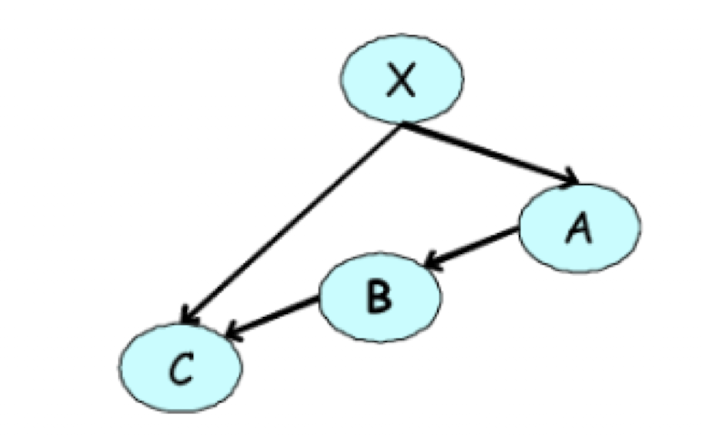
\includegraphics[width = .7\linewidth]{figures/section3/figure_3_1.png}
        \caption{An example of Sum-product inference}
        \label{fig:sum-product}
    \end{figure}
    \text{}\\
    To express the joint distribution, we introduce the nonnegative factors $\psi$: 
    \begin{align*}
        p(A, B, C) & =\sum_X p(A,\:B,\:C,\:X)\\
        & =\sum_X p(X) p(A \mid X) p(B \mid A) p(C \mid B, X) \\
        & =\sum_X \psi_1(X) \psi_2(A, X) \psi_3(A, B) \psi_4(X, B, C) \\
        & =\psi_3(A, B) \sum_X \psi_1(X) \psi_2(A, X) \psi_4(X, B, C) \\
        & =\psi_3(A, B) \tau(A, B, C)
    \end{align*}
    We eventually end with a new factor $\tau$ and it is an example of how sum-product algorithm works.
\end{example}
In general, we compute the the conditional distribution $p(x_F\mid x_E)$ using the \textbf{sum-product algorithm}. Denote $\mathcal{F}$ as the set of potentials or factors.
$$p\left(x_F \mid x_E\right) \propto \tau\left(x_F, x_E\right)=\sum_{x_R} \prod_{C \in \mathcal{F}} \psi_C\left(x_C\right)$$
For DAGMs, $\mathcal{F}$ is $\{i\}\cup\text{parents(i)},\:\forall\:\text{nodes i}$\\
For MRFs, $\mathcal{F}$ is all maximal cliques.\\
\newline
We will see more about exact inference on \hyperref[sec:message-passing]{message passing}